\section{introduction to thermal modeling and dark silicon }
In this section, we will introduce the feature of dark silicon, and then thermal modeling method will be talked about next. At the last part, task migration and DVFS will be presented.
\subsection{Feature of Dark Silicon} 
  Today's microprocessors have been in an age that not only one cores are integrated in one chip for a long time. Parallel computing enhances the performance of many-core microprocessors. However, with technology scaling and the higher and higher power density, especially for the static power or leakage power, integrated chips have meet the time that cores of a microprocessor cannot be powered on at the same time \cite{MS:DAC'2014}, as high temperature means low performance and low reliablity and the leakage power has occupied a large fraction of the whole power consumption.  



\subsection{Thermal modeling}
Based on the similarity between electronic behavior and thermal behavior, we can also use the MNA (modified nodal analysis) to simulate the thermal behavior of a chip. Temperatures of the cores are the highest among all the other parts and influence the performance of the microprocessor most. So we only care about the cores' temperature.
 And then we use the Euler's method to discrete the continuous time equation to fixed timestep \cite{MaWang:APCCAS'14} as 
\begin{equation}
\begin{split}\label{od}
t_{a}(k+1)&=A_mt_{a}(k)+B_mp(k),\\
t_{c}(k)&=C_{c}t_{a}(k).
\end{split}
\end{equation}
In \eqref{od}, take one $m-$cores chip for example, and $n$ means the number of all the thermal parts of the chip.  $t_{a}\in R^{m\times 1}$ means the temperature of all the parts of the microprocessor. $A_m \in R^{m\times m}$ and $B_m\in R^{m\times m}$ is the parameter matrix which contains information of thermal condutance, thermal capacitance and the topology of the microprocessor. $p(k)\in R^{m\times 1}$ means the power input at time step $k$, while $C_{c} \in R^{n\times m}$ means the selection matrix to select the cores' temperature from $t_{a}$ and the entries of $C_{c}$ is $1$ or $0$. $t_{c}(k)\in R^{n\times 1}$ means the cores' temperature at timestep $k$. 


 As there are only $k$ cores active in dark silicon situations, the power at time step $k$ must have zero entries. Suppose that at time step $k$, only $j$ cores are active, $j<n$ then $p(k)$  can only have $j$ nonzero entries. And in our work, we cannot still make all the cores open. However, our method can maximize the power of the active cores to some extent, without triggering the dynamic thermal management without theoretical guidence, which we will talk about later.

\subsection{Power Budgeting Method}


As the density of leakage power increases without control, it may only be possible to power on a fraction of cores for a microprocessor. There exists many distributions of active cores and different distributions leads to different temperature profile, different power upper limit and different performance.
A power budgeting method is to assign the suitable tasks to the right cores, in other words, to find the best distribution of the power. And the power budgeting method is used to guide the dynamic thermal management. 
The goal of power budgeting method is to maximize the power the chip can endure under the safe temperature constraint.


A very high temperature means a very low performance, and a very low temperature means a very high potential of performance. So we believe that there exists one temperature that maximizes the performance. And we choose it as safe temperature. And we hope that by using our new power budgeting method, the active cores' temperature is close to the safe temperature. There is one work \cite{Pagani'14} based on thermal safe power. However, \cite{Pagani'14} computes the power constraint on state conditions. When dealing with transient simulations, the power is too pessimistic. Our work use model predictive method to predict the ideal power distribution and guide dynamic thermal management and the work is suitable for transient situations.



\subsection{Dynamic Thermal Management}

The number of transistors integrated in one chip is growing and the fraction of static power occupies in the whole power consumption of a transistors is also increasing, with the technology scaling. High power density leads to high temperature, low performance.
 Based on this reason, dynamic thermal management has been used for a long time. The most two useful and famous methods are task migration and DVFS. 


 In the consideration of performance, lifetime, reliability, dynamic thermal management such as DVFS and task migration have been used to handle this problem. Dynamic thermal management lowered the maximum temperature of the chip, but still cannot change the situation  that a fraction of the cores are dark, which means inactive, because the leakage power exists once the cores are open.

For a multi/many-core system or chip, thermal sensors monitor \cite{WangTan:ICCAD'11} the temperature of the cores. If a high temperature is detected, the corresponding task which causes the high temperature will be moved to a low temperture core. As Fig. \ref{task} shows, red color means the dangerous temperature, and the temperature decreases with color red,yellow,blue. Blue color means low temperature. The sensor detects that core 5 reaches the dangerous temperature, then task migration takes effect to exchange its task with core 9.  And we can see that after using task migration, both the temperature of core $5$ and core $9$ are in the middle temperature.
 However, the mean drawback of task migration is that without prediction, it occures only when high temperature has been reached and the performance has been lowered. And for most cases, heavy tasks cause high temperatures unless task migration performs frequently, which is unprefitable for the performance.
\begin{figure}
  \centering
     {
       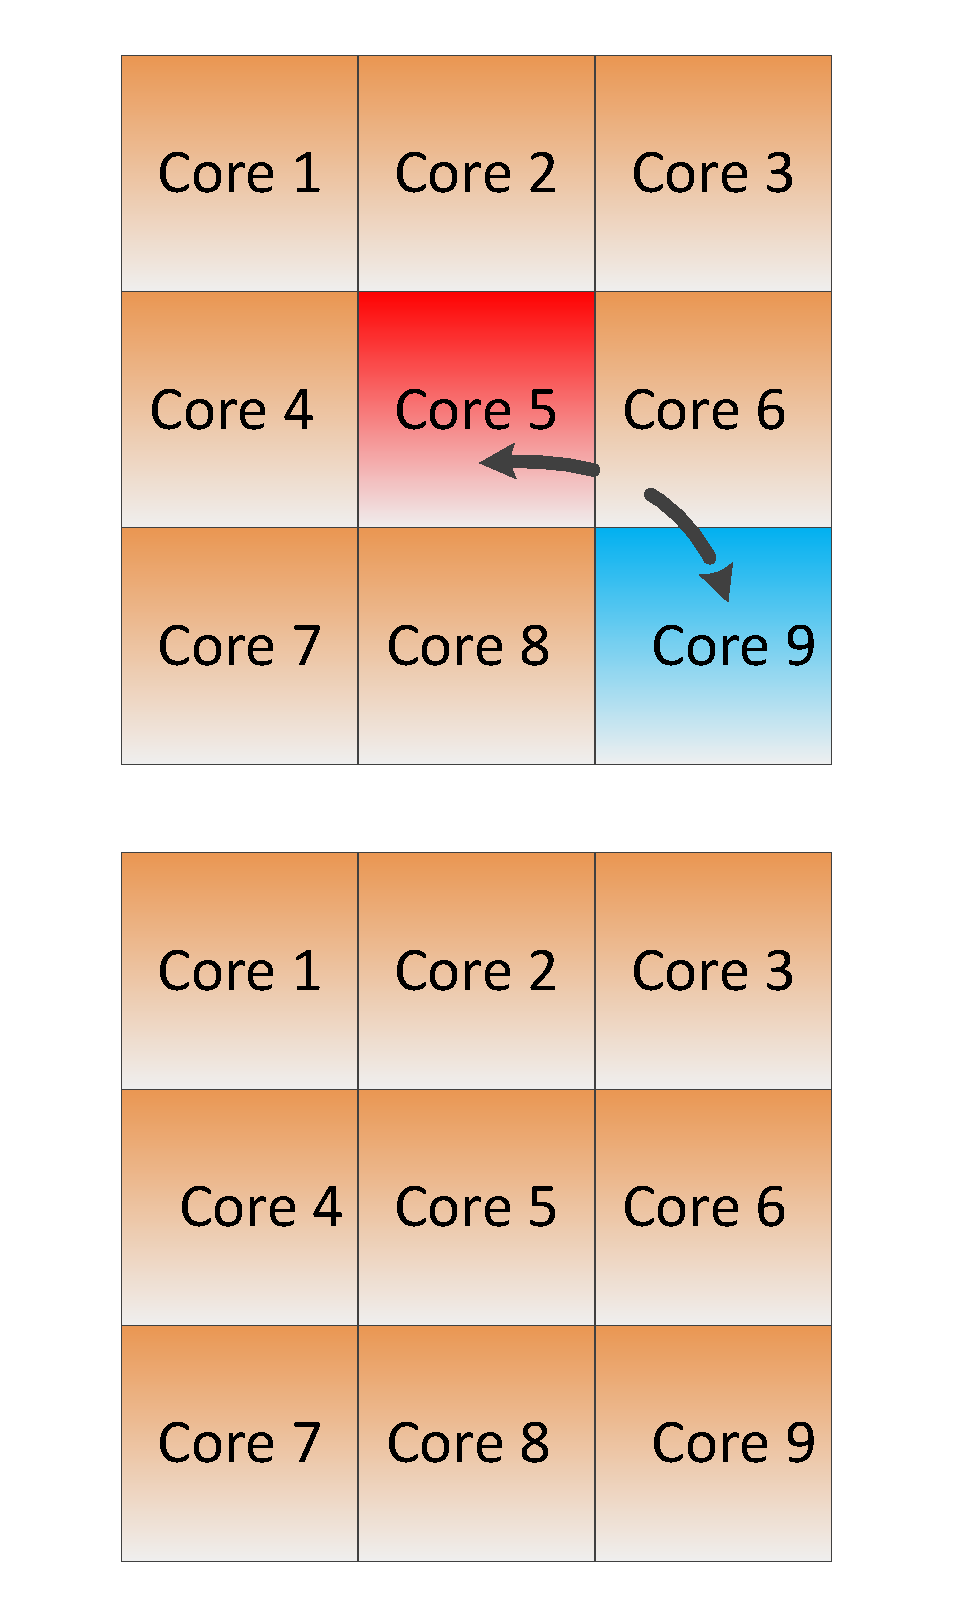
\includegraphics[width=0.4\textwidth]{fig/task}
     }
     \caption{Example of task migration}\label{task}
\end{figure}
\begin{figure}
  \centering
     {
       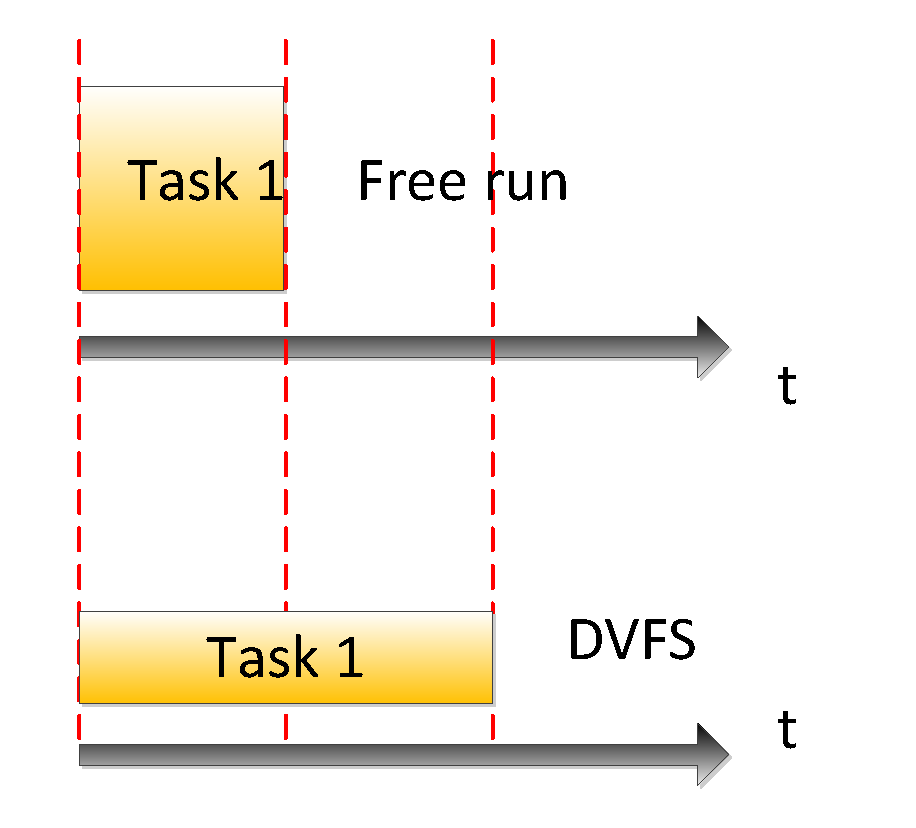
\includegraphics[width=0.4\textwidth]{fig/DVFS}
     }
     \caption{Example of task migration}\label{DVFS}
\end{figure}


In contrast, DVFS can be used in both one-core and multi/many-core systems. Once a high temperature is detected, the voltage and frequency of the corresponding cores will be lowered. Then the temperature will be lowered. It still cannot avoid the presence of hotspots. And the performance of the cores will suffer a great loss. As Fig. \ref{DVFS} shows, we use the area of the rectangle to represent the task, the height of the rectangle to represent the power consumed, and the length to stand for the time. We can see that once DVFS was performed, the task execution time will be longer.

